\documentclass[11pt]{article}
\setlength{\topmargin}{-.5in}
\setlength{\textheight}{9in}
\setlength{\oddsidemargin}{.125in}
\setlength{\textwidth}{6.25in}



\usepackage{tikz}
\usetikzlibrary{shadows,arrows}
% Define the layers to draw the diagram
\pgfdeclarelayer{background}
\pgfdeclarelayer{foreground}
\pgfsetlayers{background,main,foreground}
 
% Define block styles  
\tikzstyle{materia}=[draw, fill=black!10, text width=6.0em, text centered,
	minimum height=1.5em,drop shadow]
\tikzstyle{myNode} = [materia, text width=8em, minimum width=10em,
	minimum height=3em, rounded corners, drop shadow]
\tikzstyle{texto} = [above, text width=6em, text centered]
\tikzstyle{linepart} = [draw, thick, color=black!50, -latex', dashed]
\tikzstyle{line} = [draw, thick, color=black!50, -latex']
\tikzstyle{ur}=[draw, text centered, minimum height=0.01em]
 
% Define distances for bordering
\newcommand{\blockdist}{1.3}
\newcommand{\edgedist}{1.5}

\newcommand{\myNode}[2]{node (p#1) [myNode]
	{{#2}}}

% Draw background
\newcommand{\background}[5]{%
	\begin{pgfonlayer}{background}
		% Left-top corner of the background rectangle
		\path (#1.west |- #2.north)+(-0.5,0.5) node (a1) {};
		% Right-bottom corner of the background rectanle
		\path (#3.east |- #4.south)+(+0.5,-0.25) node (a2) {};
		% Draw the background
		\path[rounded corners, draw=black!50, dashed]
			(a1) rectangle (a2);
		\path (a1.east |- a1.south)+(0.8,-0.3) node (u1)[texto]{\scriptsize {#5}};
	\end{pgfonlayer}}




\begin{document}
\title{\textbf{Twitter Crowd Translation -- Design and Objectives}}
\author{
Eduard \v{S}ubert\\
Faculty of Nuclear Sciences and Physical Engineering\\
Czech Technical University in Prague
\and
Ond\v{r}ej Bojar\\
Institute of Formal and Applied Linguistics\\
Faculty of Mathematics and Physics\\
Charles University, Prague, Czech Republic
}

\renewcommand{\today}{June 20, 2014}
\maketitle

\def\footurl#1{\footnote{\tt{} #1}}
\def\equo#1{``#1''}

\def\hashtag#1{\texttt{\##1}}

\def\Sref#1{Section~\ref{#1}}
\def\Fref#1{Figure~\ref{#1}}

%\renewcommand{\today}{June 30, 2009}
\maketitle
%
\section{Introduction}

This paper presents Twitter Crowd Translation (TCT), our project aimed at
development of an online infrastructure serving two
purposes:
(1) providing online translation to social media and (2)
gathering relevant training data to support machine translation of such content.
We focus on Twitter and the open-source machine translation toolkit
Moses. Our project heavily relies on unpaid voluntary work.

In \Sref{motiv}, we provide the motivation for both goals of our work.
% Tohle zatim nemame, ale v plnem clanku by to byt melo:
%\Sref{chall} briefly lists the challenges specific to machine translation of
%social media, focusing more on the technical aspects than on the inherent
%linguistic characteristics concerning style, register etc.
\Sref{design} describes the overall design of our tool in terms of
\equo{social engineering} and \Sref{implementation} complements it by the
technical aspects.

% for creation and
% maintenance of corpora for machine translation without the need of hiring
% translators while using the power of crowd instead. The application is designed
% to be able to work with any source phrases; however we specialize for
% translation of tweets from popular social network Twitter.
%
%The aim of our project is to create and maintain corpora for machine
%translation without the need of hiring expensive translators while using the
%power of crowd instead. We achieve this with online interface which allows
%addition of new phrases to corpus their translation as well as evaluation of
%the best translation. Aside from creating the corpus application offers
%language practice and access to foreign content to users.

\section{Motivation}
\label{motiv}

Social networks have gained tremendous popularity and 
have successfully replaced many established means of communication. 
While geographical location of the users has little to no impact on 
communication, the obstacle of \emph{languages used} remains.
% stejne bych spis rekl: languages spoken

For stable and long-lasting content, the problem is less severe:
services such as the Wikipedia have shown that
volunteers are able to provide translations into many languages. 
Machine translation is easy to train on such
content and delivers moderately good results.

On the other hand, social networks are used in a streaming fashion, Twitter
being the most prominent example. Anybody can contribute message, 
which is forwarded to a number of followers. These, in turn, are flooded 
with messages from sources they select. Given the constant flow
of new information, nobody looks back at older messages.
% the expiration time of a single message is short.

Providing translation to \equo{streaming networks} is much more challenging.
The input is much noisier, significantly reducing MT output quality, and the
community is less interested in providing manual translations.

The social motivation of our project is to break the language
barrier for streaming social networks. The technological motivation is to
advance MT quality by collecting more and better-fit data.
What Wikipedia and on-line MT services manage for stable content,
we would like to achieve for streaming networks and casual, unedited content.

\section{Design of TCT}
\label{design}

We see two main reasons for people to 
contribute to community translation of Wikipedia and other projects: sharing the information 
(\equo{What is useful for me in my language may be useful for others.}), 
and self-promotion
(\equo{I will gain good reputation by contributing well received translations.}).
We designed our project in accordance to these findings.

TCT should be as thin layer as possible, to cause 
minimal disruption. 
The majority of users stay within their platform -- Twitter in this
case.

To better explain the processes of TCT, we assign users roles: 
%We describe the process in terms of roles users take:
\textbf{Author}, \textbf{Selector}, \textbf{Translator}, \textbf{Judge} 
and \textbf{Recipient}.

\Fref{schema} summarizes the workflow: a tweet in a foreign language is
posted by \textbf{Author} and observed by a \textbf{Selector}. 
The \textbf{Selector} does not fully understand the message 
and submits it for translation to the language of his choice. 
Our TCT server collects this request and
forwards it to human and machine \textbf{Translators}. Translations 
are collected and \textbf{Judges} evaluate their quality, high-confidence
machine translation might bypass this step. The best
translation is tweeted to \textbf{Selector} and other \textbf{Recipients} 
by our server. 
The same user can take several roles in the process. 

\begin{figure}[h]
\begin{center}


\begin{tikzpicture}
	
	\path \myNode {1}{\textbf{Author:}\\ phrase};
	\path (p1.south)+( 0.0,-1.0) \myNode{2}{\textbf{Selector:}\\ \texttt{\#tctrq} phrase};
	\path (p1.south)+( 5.0,-1.0) \myNode{3}{\texttt{Collects the message}};
	\path (p1.south)+(10.0,-1.0) \myNode{4}{\texttt{Notifies the translators}};
	\path (p3.south)+( 0.0,-1.0) \myNode{5}{\texttt{Machine translation}};
	\path (p5.south)+( 5.0,-1.0) \myNode{6}{\textbf{Translator:}\\ translation};
	
	\path (p5.south)+( 0.0,-1.0) \myNode{7}{\texttt{Collects translations}};
	\path (p7.south)+( 0.0,-1.5) \myNode{8}{\textbf{Judge:}\\ compares translations};
	\path (p7.south)+(-5.0,-1.5) \myNode{9}{\texttt{Publish best translation}};

	\path (p9.south)+( 0.0,-1.0) \myNode{10}{\textbf{Recipient}};
	
		 
	% Draw arrows between elements
	\path [line] (p1.south) -- node [above] {} (p2);
	
	\path [line] (p2.east) -- node [above] {} (p3);
	
	\path [line] (p3.east) -- node [above] {} (p4);
	\path [line] (p3.south) -- node [above] {} (p5);
	
	\path [line] (p4.south) -- node [above] {} (p6);
	\path [line] (p5.south) -- node [above] {} (p7);
	
	\path [line] (p6.west) -- node [above] {} (p7);
	
	\path [line] (p7.south) -- node [above] {} (p8);
	\path [line] (p8.west) -- node [above] {} (p9);
	
	\path [line] (p9.south) -- node [above] {} (p10);
	
	\background{p1}{p1}{p10}{p10}{}
	\path (p1.north) node (u1)[texto]{Twitter};
	\background{p3}{p1}{p8}{p10}{}
	\path (p3.north)+(0.0,1.5) node (u2)[texto]{TCT system};
	\background{p4}{p1}{p6}{p10}{}
	\path (p4.north)+(0.0,1.5) node (u3)[texto]{Mail};
	
\end{tikzpicture}


\end{center}
\caption{Twitter Crowd Translation in a nutshell.}
\label{schema}
\end{figure}

We think that each of the user groups profits from using TCT. 
\textbf{Author} gains bigger audience. 
\textbf{Selector} achieves full understanding of the tweet.
\textbf{Translator} and \textbf{Judge} practice their language skills 
and \textbf{Translator} is placed in the TCT hall of fame.
Finally \textbf{Recipient} gains more of understandable content.

\section{Technical Aspects of TCT}
\label{implementation}
% It is important for us to let users interact with TCT through their platform.
%Most users should interact with TCT through their platform.
To remain in the Twitter platform,
\textbf{Selector} submits messages as tweets marked with hashtag 
\hashtag{tctrq} and TCT uses Twitter REST API to search twitter feed
for such tweets.

Once tweets are collected, \textbf{Translators} are notified via e-mail
to which they respond with translations. % and TCT collects received e-mails.

\textbf{Judges} are %the only group that is
required to contribute via 
TCT website and evaluate the quality of translations by blind one-to-one 
comparison. 

An interesting feature is password-less registration. 
Translators are the only group required to register but their interaction
is strictly e-mail based, all necessary settings are accessed by expiring links sent via e-mail on request. 

\section*{References}

% \bibliography{biblio}
% \bibliographystyle{plain} 

\paragraph{Moses} - http://www.statmt.org/moses/
\paragraph{Twitter} - http://twitter.com/

\end{document} 
